% Chapter Template

\chapter{Working Environment} % Main chapter title

\label{Chapter2} % Change X to a consecutive number; for referencing this chapter elsewhere, use \ref{ChapterX}

\lhead{Chapter 2. \emph{Working Environment}} % Change X to a consecutive number; this is for the header on each page - perhaps a shortened title

%----------------------------------------------------------------------------------------
%	SECTION 1
%----------------------------------------------------------------------------------------

\section{UCL's wireless infrastructure}

<<<<<<< HEAD
The university also owns several student campus. The headquarters of the UCL is located in the city of Louvain-la-Neuve. The campus gathering the health sciences is located in Woluwe-Saint-Lambert and more recently the cities of Tournai and Mons as well as Charleroi were added to the list.

Faced with such a scale, it is vital for the Catholic Univeristy of Louvain to develop a reliable and efficient Internet connection and wireless network able to deliver a connectivity throughout its campus and all users at all time.

The purpose the University enrolled in is to provide an Internet access and a connectivity according to the type of user who wants to connect. To do this, there are 3 main networks at the Catholic University of Louvain, each with a different SSID.

The univeristy also participates in the projet \texttt{eduroam} (which stands for education roaming). Eduroam is the secure, world-wide roaming access service developed for the international research and education community\cite{eduroam1}.
=======
\subsection{Overview}
On its Louvain-la-Neuve's campus area, the Catholic University of Louvain offers 4 different networks, with different SSIDs, that are reserved to certain parts of users according to their category. Those available networks are the following:
\begin{itemize}
	\item[-] \texttt{student.UCLouvain}: Available for the students enrolled at UCL.
	\item[-] \texttt{UCLouvain}: Reserved for university's professors and the researchers.
	\item[-] \texttt{UCLouvain-prive}: Limited access to check the UCL's wireless configuration page or to download required program for Windows XP and Vista.
	\item[-] \texttt{visiteurs.UCLouvain}: Accessible for guests invited by the university.
	\item[-] \texttt{eduroam}: Internation education roaming access.
\end{itemize}

Security is an important issue at the university and several measures are regularly taken by the SRI team in order to keep the integrity and the consistency of the UCL's network untouched. As an example, Windows has decided on the 8th of April 2014 to end the XP's support and updates leaving all the remaining laptops running this operating system unprotected to possible external threats\cite{windows}. The problem with that Windows' decision is that those computers might become more vulnerable to security risks and viruses and if a contaminated host connects to the UCL's network it can cause serious damages to the overall infrastructure depending on what the virus is programmed to do. This is why the SRI team took the decision to block the wireless access to any device that still uses Windows XP after the 8th of April.

The main way of protecting the network infrastructure from possible threats that has been installed and configured by the SRI team is the use of the IEEE 802.1X standard providing an authentication mechanism for the devices that want to connect to a UCL's network.\\
Basically, every student, professor or researcher needs a special WiFi username and a password to connect to one of the networks. The username is composed of two parts, on one side the general login the user has received from the university's administrative system when he had enrolled himself, and on the other side the following part \texttt{@wifi.uclouvain.be}. With that username, the user also needs a password, which is the same has the password he uses to connect to the university's web site. Without those credentials or if the user misspell he's username or password, it is impossible for him to connect to the UCL's wireless network.

This kind of authentication mechanism is only possible if the infrastructure has several key entities that are going to handle all of this security process.
>>>>>>> 8550f8c6dbce76fe0c7794f2fbf34175366b032e




<<<<<<< HEAD
\section{Hardware infrastructure}
Using the network monitoring software InterMapper\cite{intermapper} we see that the UCL network is composed of seven neighborhood routers (CtPythagore, CtHalles, CtLew, CtStevin, CtCarnoy, CtMichotte and CtSH1C). Six of them are present on the Louvain-la-Neuve campus and only CtLew is on the Wolluwé Campus. Those routers task is only routing.
=======
\subsection{Design}
Using the network monitoring software InterMapper\cite{intermapper} we see that the UCL network is composed of seven neighborhood routers (CtPythagore, CtHalles, CtLew, CtStevin, CtCarnoy, CtMichotte and CtSH1C). Six of them are present on the Louvain-la-Neuve campus and only CtLew is on the Wolluwé Campus. Those routers task is only routing.\\
>>>>>>> 8550f8c6dbce76fe0c7794f2fbf34175366b032e

Internet access is provided by Belnet via a 10GBit ethernet link directly connected to the CtPythagore. There is also a second 3GBit ethernet link connected to the CtHalles router but this link is never used. It is only a backup link in case of failure of the main one.

The infrastrucutre also has two main servers which are CtTier2 and CtAquarium. Those main servers are datacentres that contain the RADIUS servers as well as the LDAP servers.

Then for each building there is a switch and this switch is directly connected to one of the seven routers. Each of those switches has 48 ports that are connected to the access points inside the concerned building.\\
Concretely, in each building we find ethernet plugs that are connected to what we call concentration points. Those points contain commutators that is connected to the building switch that is connected to one of the main routers.\\
An important point to mention is that the network is not a full mesh.

Here is a simplified representation of the UCL network infrastructure:
\begin{figure}[H]
	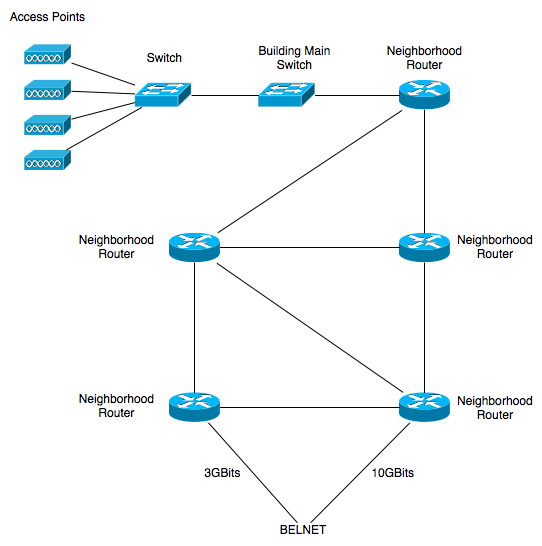
\includegraphics[width=.9\linewidth]{Pictures/Chapter2/infrastructure.png}
\end{figure}

\section{Network Topology}
Here is the representation of the network topology:
\begin{figure}[H]
	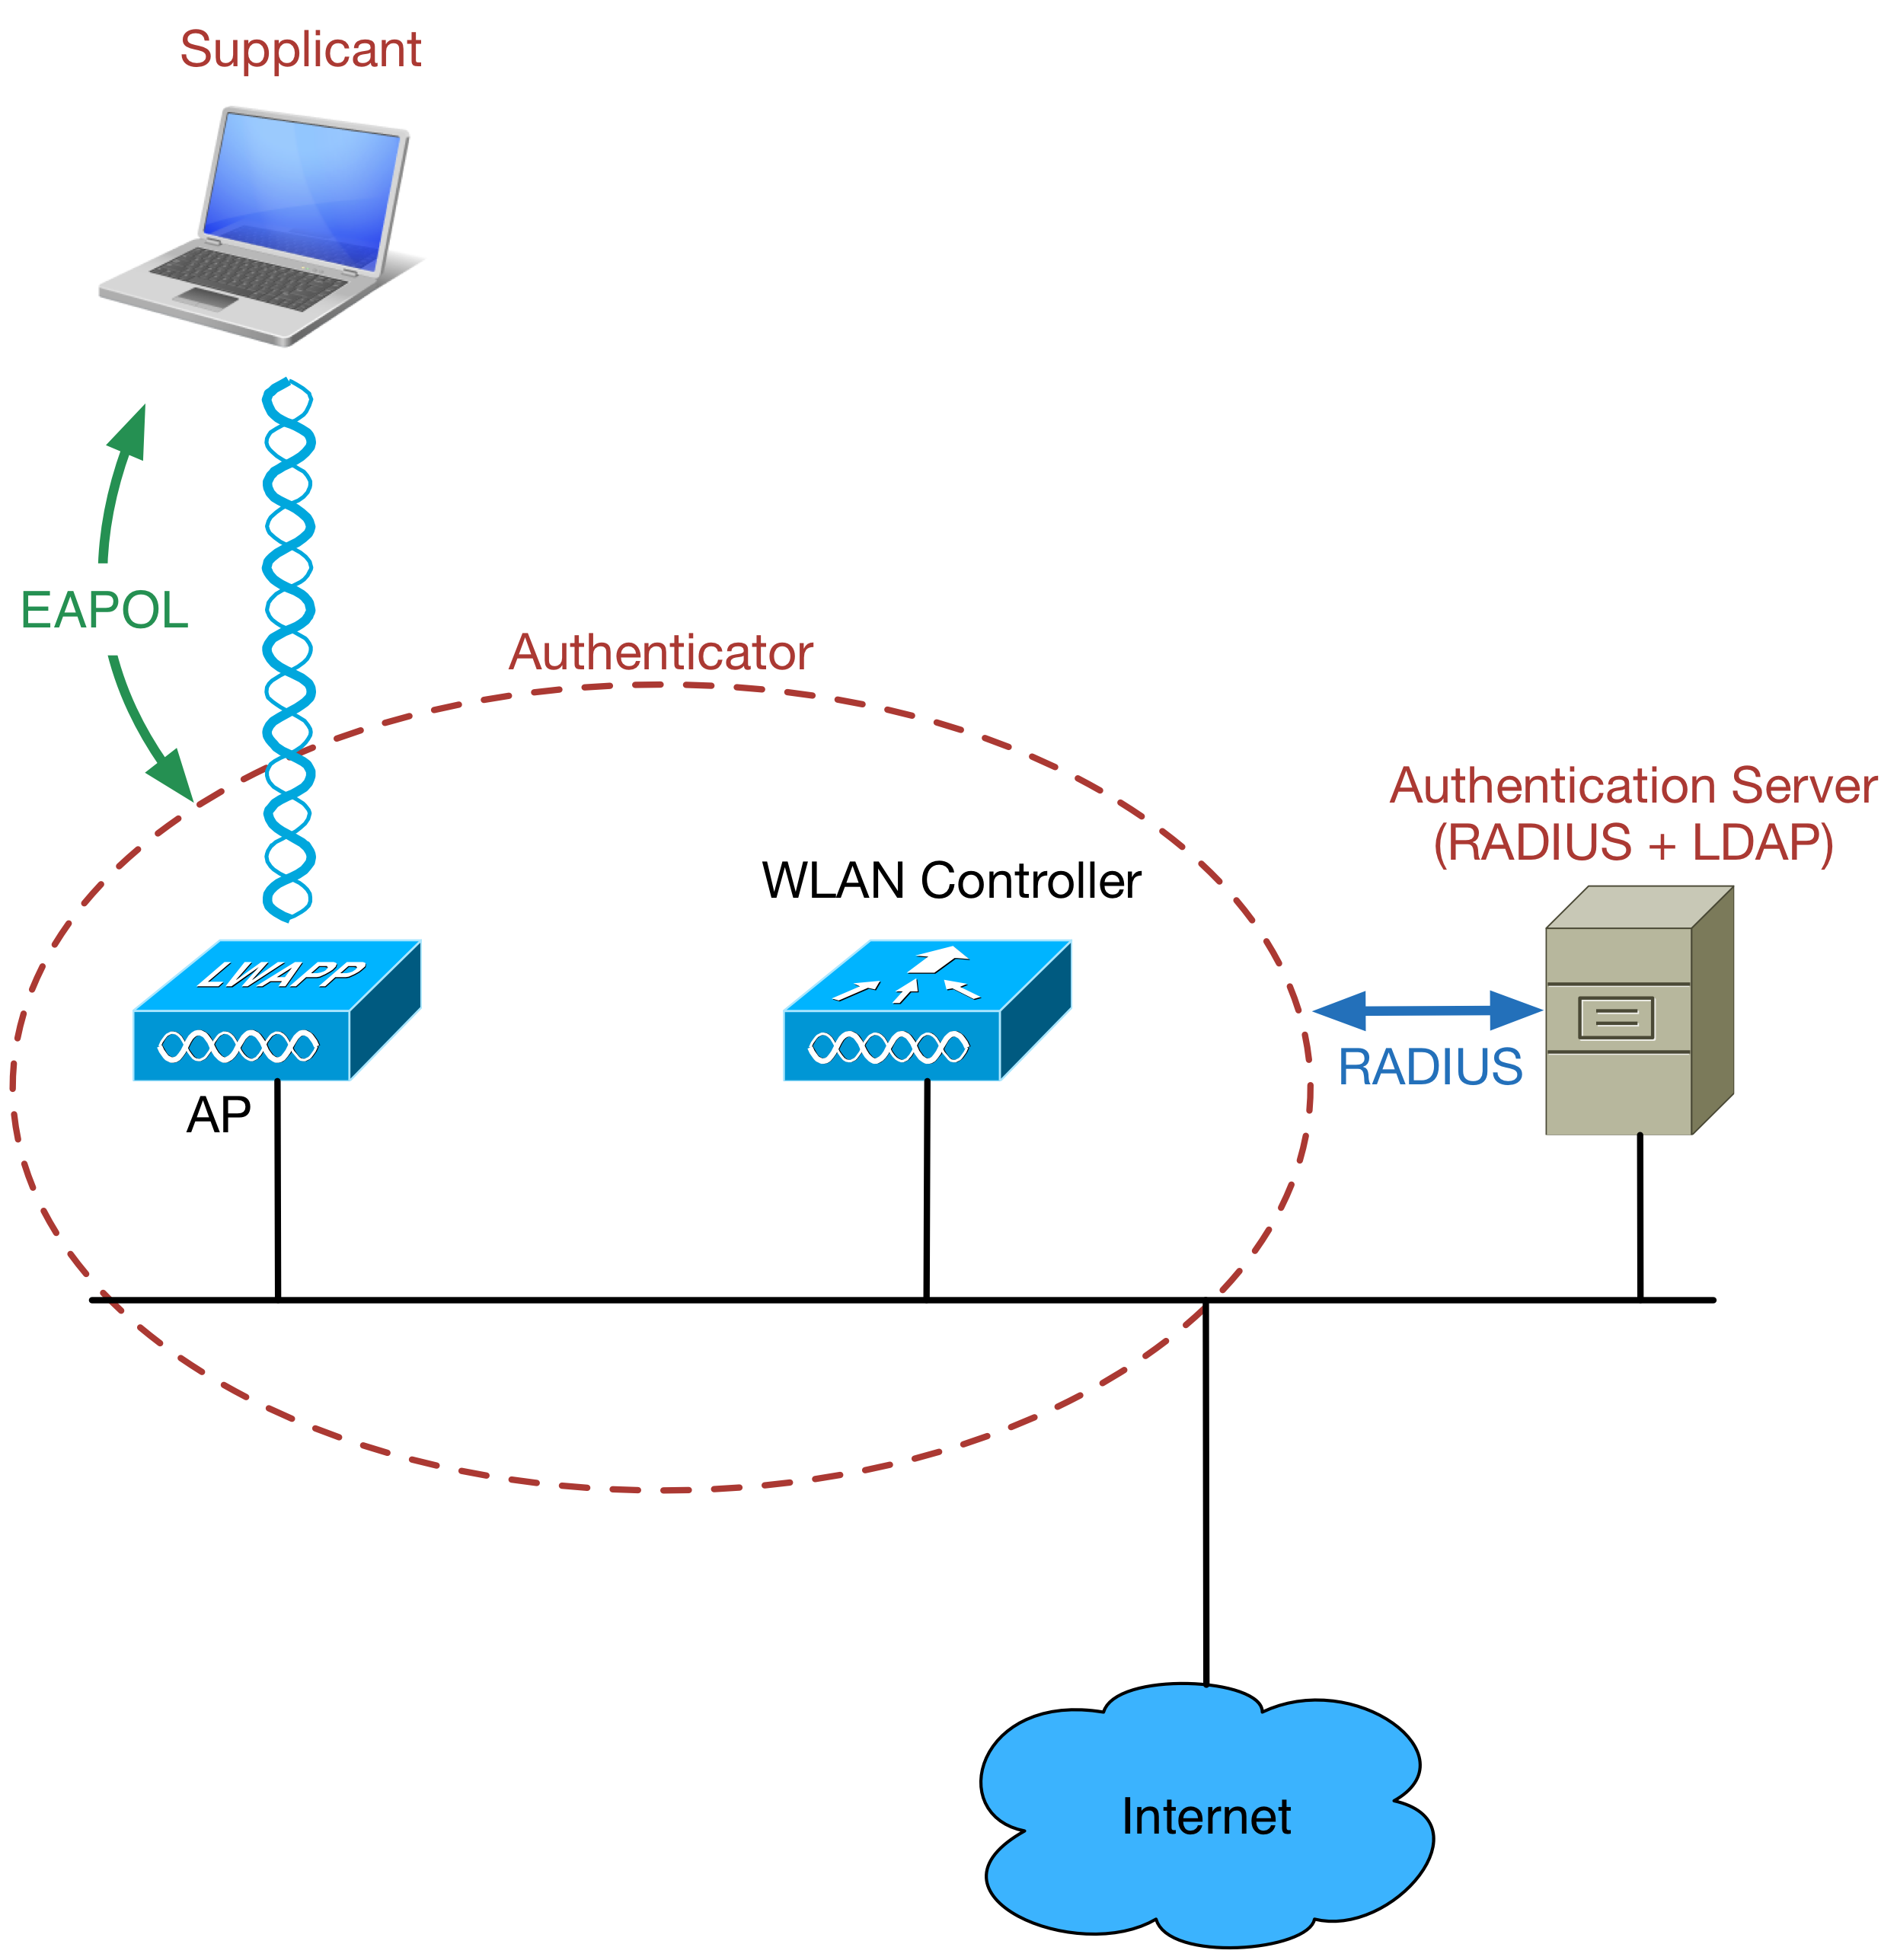
\includegraphics[width=.9\linewidth]{Pictures/Chapter2/topology.png}
\end{figure}
The Catholic University of Louvain has chosen to use the IEEE 802.1X protocol for user authentication. Thus when a user wants to connect to the WiFi, the access point will realize an EAP negociation with the supplicant. It transmits this EAP information to the controller who is going to interact with the RADIUS authentication server who, in turn, is going to asks information to the LDAP server. Once the RADIUS server authenticate the requesting user, the connection is established.




\section{Understanding the passive and active logs}